After the panel factorization, the operation performed on the trailing sub-matrix is the update. The update takes the array of pivots produced by the panel factorization, swaps the rows and then apply \textit{trsm} and \textit{gemm} operations.

To perform one swap, the algorithm depend on the value of the pivots, this is what we call data dependency and so the algorithm is a dynamic algorithm (section \ref{task_flow_lu}). The solution to represent a dynamic algorithm with a static DAG of task flow is to make a path with all tasks. In practice, it means that all tiles must participate in swapping even if they aren't concerned.
For that, each tile will have a workspace of two arrays: the first to store one row coming from the upper tile and the second to store one row going to the upper tile. Nodes will share between them the workspaces and fill them with the appropriate rows.
The \textit{all\_reduce} seems to be the right operation to use. The cost of a \textit{all\_reduce} operation is $log_2(n_t)$. Thus, the cost of all swaps of one panel is $n_b*log_2(n_t)$. This is very expensive relatively to the cost of SPMD model which is at most $2*n_b$.
Moreover, a the end of each \textit{all\_reduce} operation, only two nodes will really use the rows collected in their workspace (the upper tile and the tile which exchange with it).

A good idea is to perform all swaps at the same time. However, this is not possible with pivots. In fact, because that the same row can be several time the maximum row, it is necessary to execute the pivots in the right order (from the first to the last). Figure \ref{fig:pivots} show an example of a row which contain twice time successively the maximum row, we can see that the row 1 go down to the row 13 then come back to the row 2. Thus, it force us to perform the first pivots before the second.

\begin{figure}[!ht]
\begin{minipage}[!ht]{.4\textwidth}
\centering
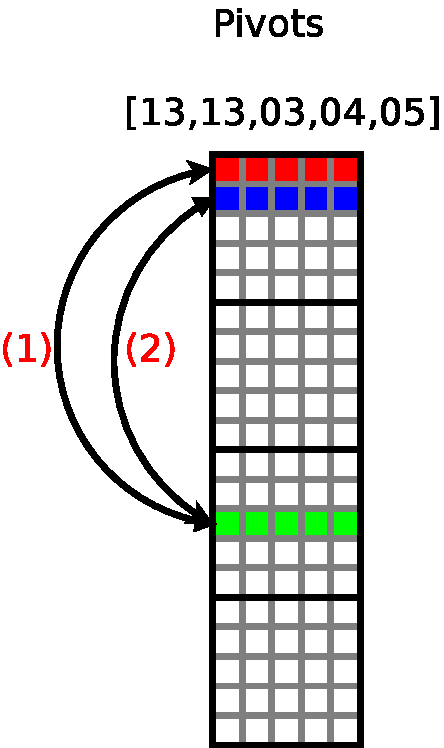
\includegraphics[height=5cm]{figures/pivots.pdf}
\caption{Row movements with pivots\label{fig:pivots}}
\end{minipage} \hfill
\begin{minipage}[!ht]{.4\textwidth}
\centering
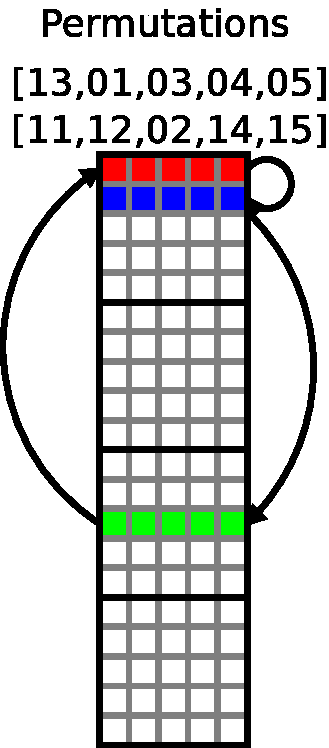
\includegraphics[height=5cm]{figures/permutations.pdf}
\caption{Row movements with permutations\label{fig:permutations}}
\end{minipage}
\end{figure}

To reduce high cost of all swaps, the key seems to use another structure instead pivots. For that, the permutations are the right solution. In fact, permutations are an array of size $n$ (we see after that it can be reduced). For each index $x$ of the array $perm$, the $(perm(x)$ row will be moved in place of the $x$ row. Thus, with permutations, we know from the beginning the final place of each row. 
Figure \ref{fig:permutations} shows the use of permutations instead pivots which is showed in Figure \ref{fig:pivots}, we can see that the row 1 go directly to the row 2 and don't move again.
Thanks to this structure, all the rows can be swapped in one single step and the cost will be just $log_2(n_t)$. 
We remark that at most $n_b$ rows go into and from the diagonal tile. Thus, the array of permutations may be limited to a size of $2*n_b$, $nb$ for permutations and $nb$ for the inverse of permutations. Therefore, instead using a workspace of two arrays, it is necessary to use two buffer of tile size for communications: the first is a copy of the upper tile, it is shared from one node to the others and each one extract from it rows needed, we will call this operation \emph{swap from}. The second buffer is to gather rows destined to the upper tile, each node create its own buffer, fill it with rows destined to the upper tile and then participate with it in a \textit{gather} operation, this operation will be called \emph{swap into}. This solution allow us to perform the \emph{swap from} and the \emph{swap into} in parallel.

Task flow \ref{fig:distributed_update_task_flow} represent the swapping operation of update operation for distributed architecture. The bold arrows shows some dependencies which add synchronizations to avoid \emph{read after write} effects. For example, the copy of the upper tile must be applied before its update.

\begin{taskflow}[!ht]
\centering
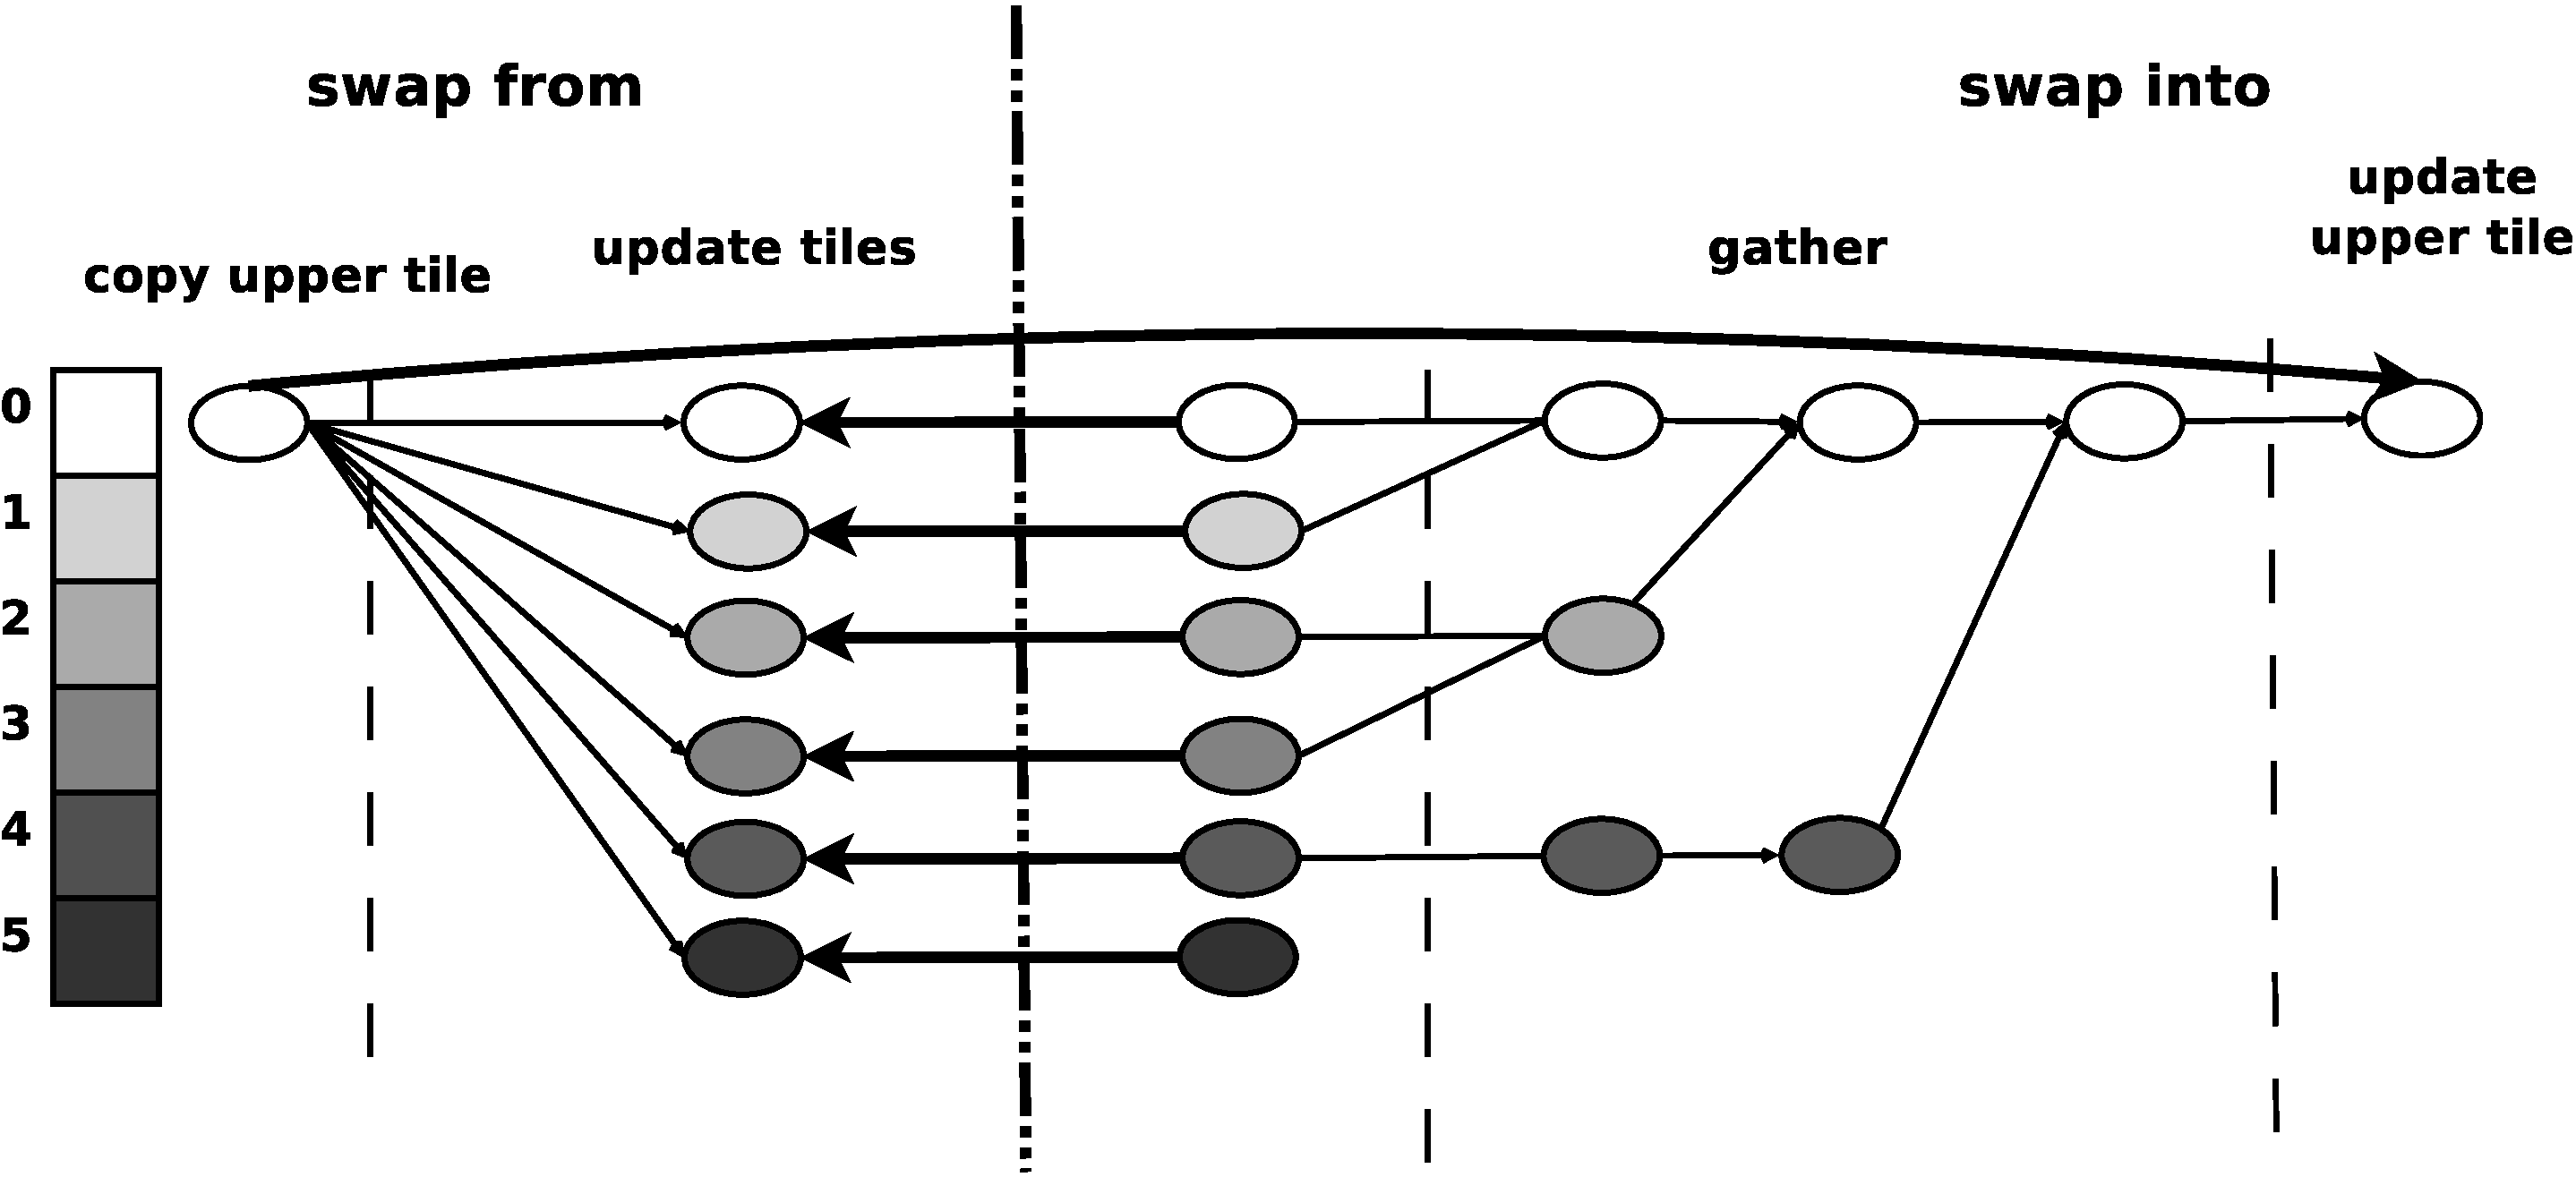
\includegraphics[width=0.8\textwidth]{figures/distributed_update_tf_bw.pdf}
\caption{Swapping operation of update on distributed architecture \label{fig:distributed_update_task_flow}}
\end{taskflow}

As for the panel factorization, we consider that nodes can be multi-core. In order to reduce global communication, each node share its buffers over its local tiles before send them to others nodes. Task flow \ref{fig:update_task_flow} show the update operation for hierarchical architecture.

\begin{taskflow}[!ht]
\centering
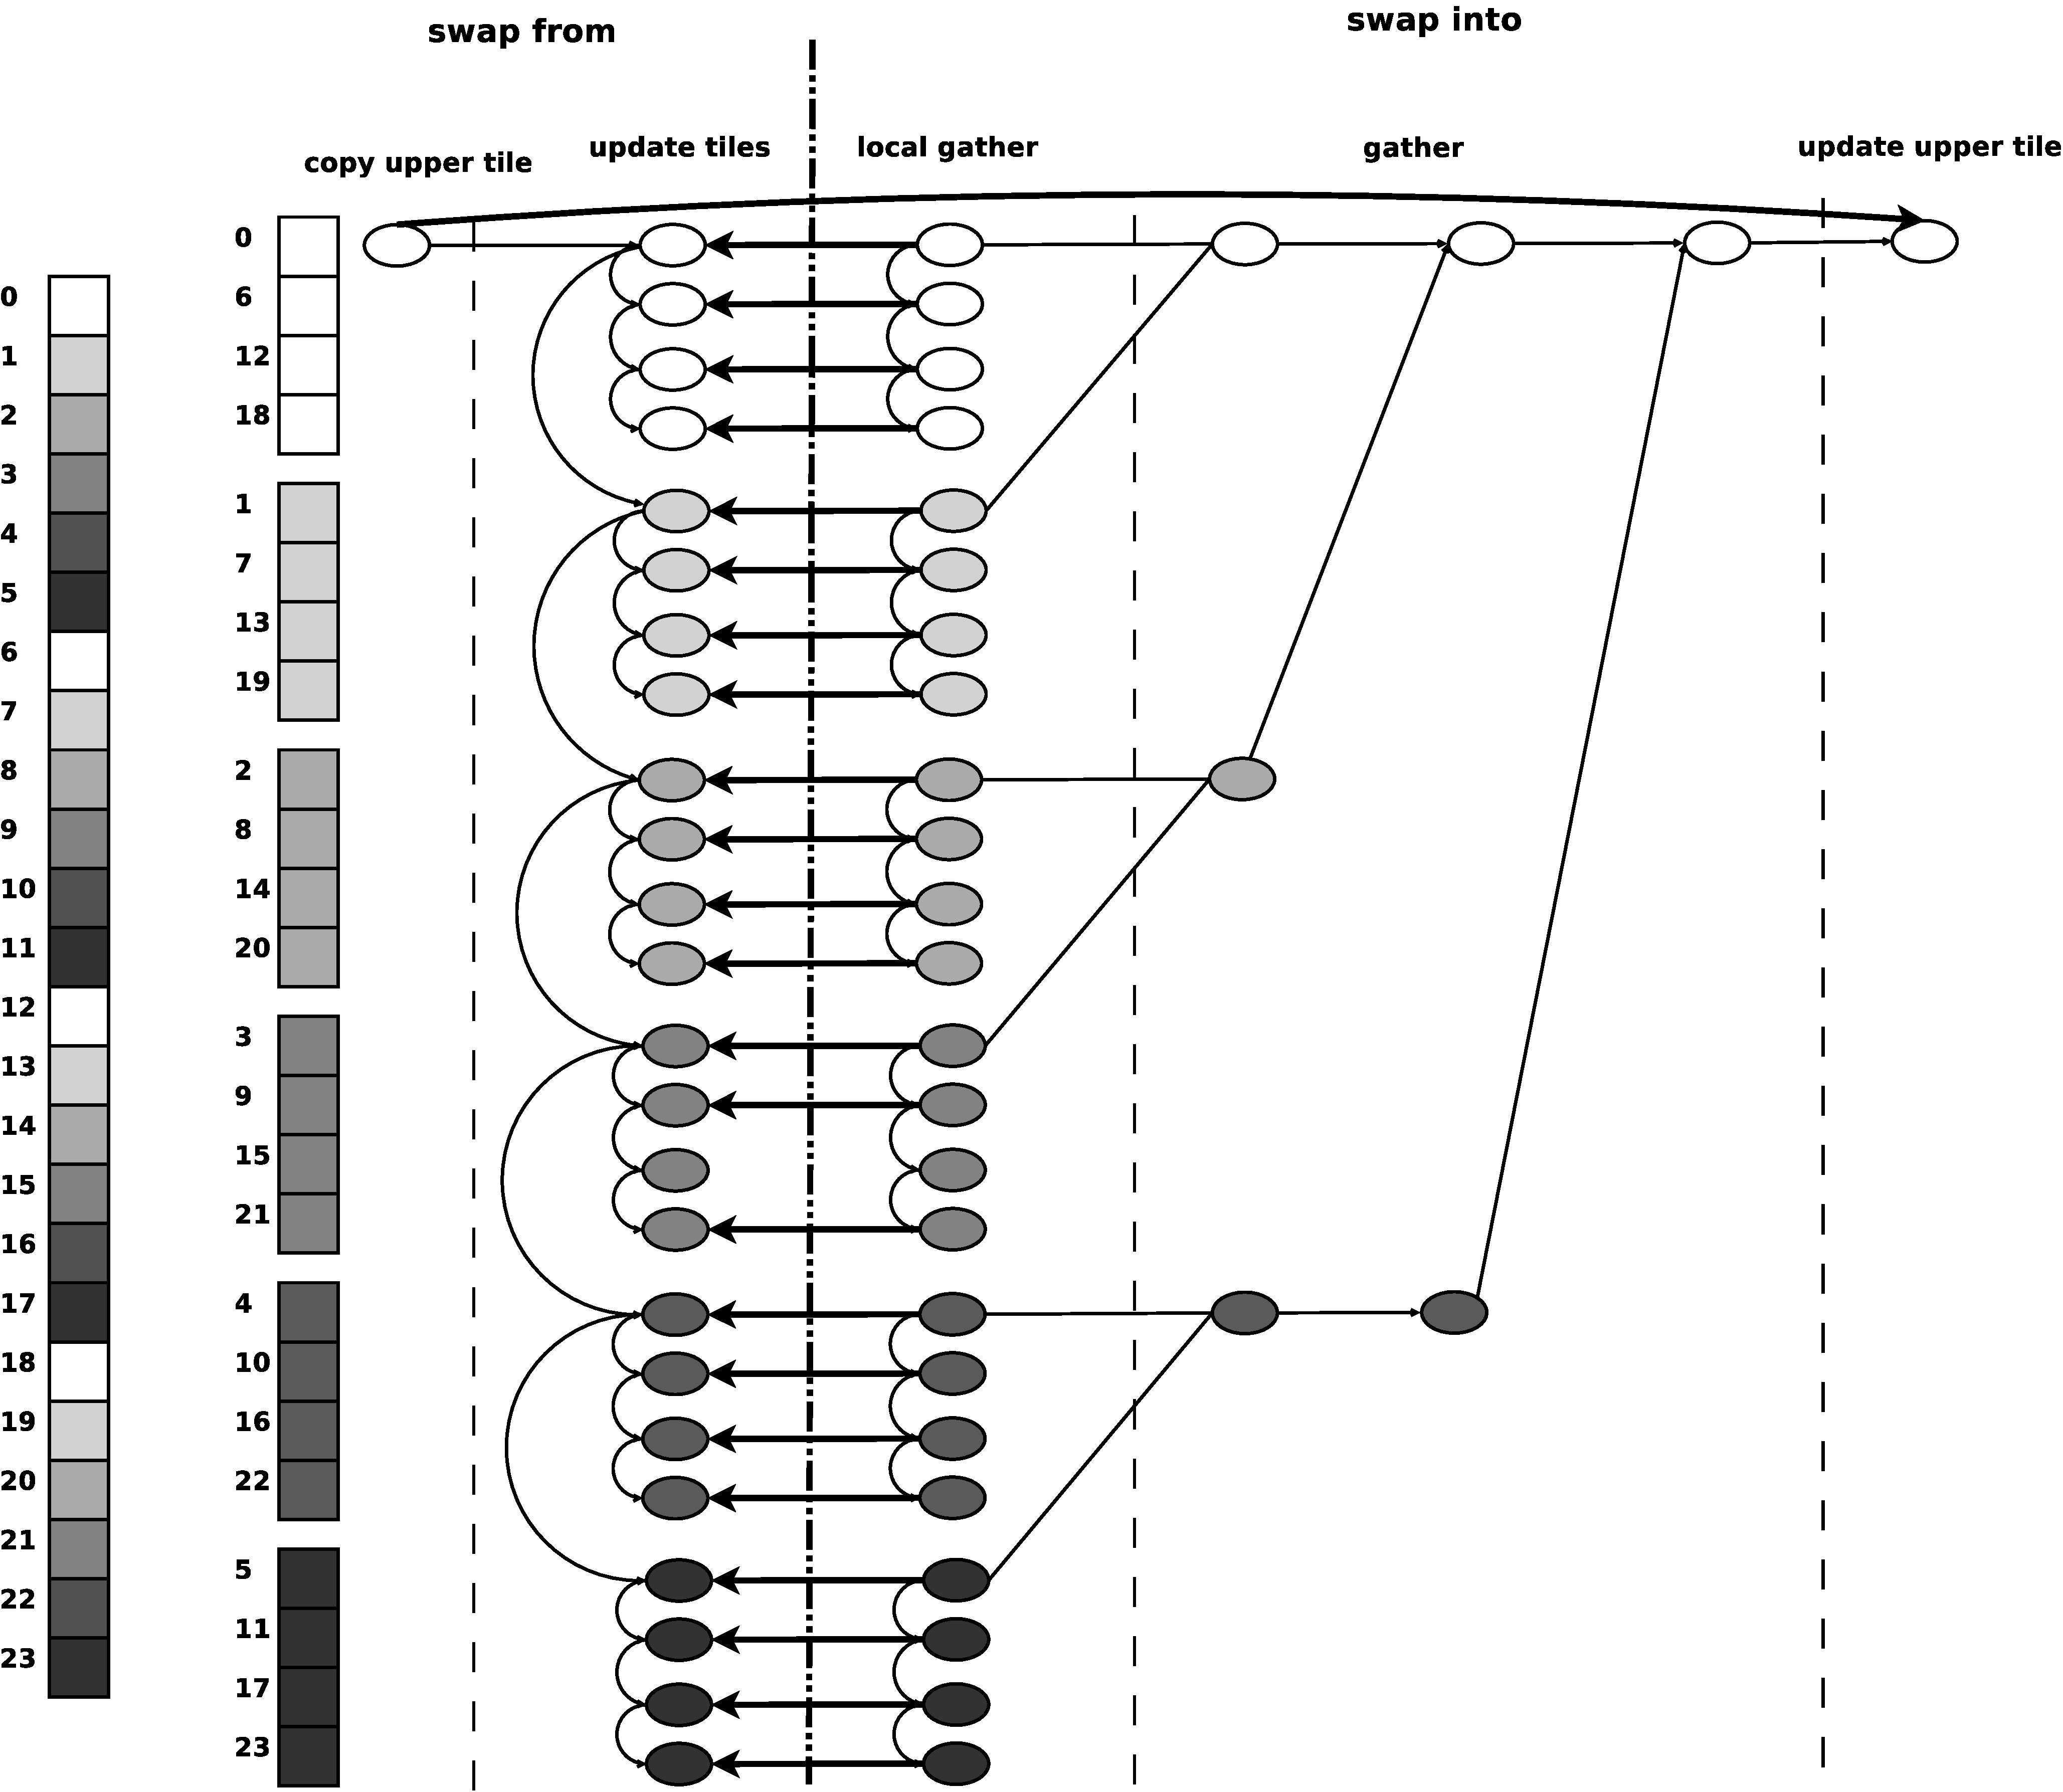
\includegraphics[width=0.8\textwidth]{figures/update_tf_bw.pdf}
\caption{Swapping operation of update on hierarchical architecture \label{fig:update_task_flow}}
\end{taskflow}

Moreover, the update engine implemented is generic because it can execute update operation after any panel factorization which provide an array of pivots.
